\chapter{Einführung} %Aufgabenstellung, Problematik und Zielsetzung der Arbeit als Vorausschau (1-2 Seiten)

\section{Einordnung der Arbeit}
Dieser Abschnitt beschreibt die Einordung der Arbeit in den Kontext des 
Projektes.

Ein elektrischer Oszillator ist eine Schaltung, die an seinem Ausgang ein
Signal mit einer bestimmten Frequenz erzeugt.

Für den Bau von elektrischen Ozillatoren gibt es verschiedene Topologien.
Zu den charakterisierenden Eigenschaften von Oszillatoren gehören neben
der Frequenz $f$ des Oszillators, die Frequenzstabilität und das Spektrum des 
Ausgangssignals.

Für ein Spektrum mit kleinen Anteilen von Frequenzen, die nicht die des 
Ausgangssignals sind, können Oszillatoren mit einer Wien-Robinson-Brücke als 
frequenzbestimmendes Element genutzt werden.

Der im Projekt verwendete Wien-Oszillator soll durch eine rauscharme 
Spannungsquelle mit der Betriebsspannung versorgt werden.
Zu den charakterisierenden Eigenschaften von Spannungquellen gehören neben der
Ausgangsspannung, das Verhältnis der Eingangsspannungsänderung zur 
Ausgangsspanngsänderung (eng.\ power supply rejection ratio — PSRR),
das Verhältnis der Änderung der Ausgangsspannung zur Änderung der Ausgangslast
(eng.\ load regulation) und das Spaktrum der Ausgangsspannung.

In der Anwendung als Spannungsversorgung eines Wien-Oszillators ist die 
Ausgangslast konstant. Die Lastregelungsfähigkeit hat also eine untergeordnete
Bedeutung. Der Oszillator soll über ein Labornetzteil mit der 
Versorgungsspannung versorgt werden. Somit können Einflüsse der 
Veränderung der Eingangsspannung minimiert werden. 

\section{Grundlagen Linearspannungsregler}
Dieser Abschnitt beschreibt die Funktion eines Linearreglers allgemein.

Eine elektrische Schaltung benötigt in der Regel eine konstante 
Versorgungsspannung um ihre Funktion zu erfüllen.
Eine Änderung der Spannung kann zur Verschiebung von Arbeitspunkten und damit
zu einer Veränderung des Verhaltens der Schaltung führen.

Um die Versorgungsspannung einer Schaltung konstant zu halten werden 
verschiedene Ansätze verwendet:

\begin{itemize}
  \item chemische Konstantspannungsquellen
  \item DCDC-Konverter
  \item Linearspannungsregler
\end{itemize}

Chemische Konstantspannungsquellen erzeugen eine Ausgangsspannung mit einer 
hohen spektralen Reinheit, da diese ihre Ausgangsspannung von anderen 
Störeinflüssen getrennt aus einer chemischen Reaktion erzeugen.
Nachteilig bei der Benutzung chemischer Quellen ist der Wartungsaufwand, der

DCDC-Konverter haben in der Regel einen hohen Wirkungsgrad über einen großen
Eingangsspannungsbereich und können je nach verwendeter Topologie auch 
Ausgangsspannungen größer als die Eingangsspung erzeugen.
Nachteilig ist, dass die Schaltfrequenz der benutzten Schalter im Spektrum der
Ausgangsspannung sichtbar ist und aufwändig gefiltert werden muss.

Linearspannungsregler haben, durch den Verzicht auf schaltende Elemente eine
hohe Spektrale Reinheit der Ausgangsspannung.
Der Wirkungsgrad eines Linearspannungsreglers hängt von der Differenz der 
Eingangsspannung zur Ausgangsspannung ab:
\[\eta = \frac{P_{\rm out}}{P_{\rm in}} \approx \frac{U_{\rm out} 
\cdot I}{U_{\rm in} \cdot I} = \frac{U_{\rm out}}{U_{\rm in}}\]
Ist die Ausgangsspannung der Schaltung nahe an der Eingangsspannung,
so ist der Wirkungsgrad hoch. Ist die Ausgangsspannung viel kleiner als die
Eingangsspannung, so ist auch der Wirkungsgrad kleiner.
Die Differenz zwischen Eingangsleistung und Ausgangsleistung geht im 
Spannungregler als Wärme verloren. 

Der Linearspannungsregler besteht sich aus einem aktiven Element, meist ein 
Bipolartransistor oder einem MOSFET, einer Regeleinrichtung und einer 
Spannungsreferenz.
Das aktive Element wird in dieser Schaltung als steuerbarer Widerstand 
eingesetzt.
Die Regeleinrichtung vergleicht die Ausgangsspannung mit der Spannung der 
Spannungsreferenz und erzeugt aus der Differenz dieser Spannungen ein 
Ansteuersignal für das aktive Element.
Die Spannungsreferenz soll die Sollspannung unabhängig von der Eingangsspannung
erzeugen.
Die Abb.~\ref{FIG:LINREG} zeigt ein Beispiel eines Linearreglers mit einem
MOSFET als aktives Element, einem Operationsverstärker als Regler und einer
Z-Diode als Referenzspannungsquelle.

\begin{figure}
  \centering
  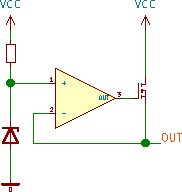
\includegraphics[clip, width=0.33\textwidth]{./../common/schaltungen/linearregler/linearregler.pdf}
  \caption{Linearregler}\label{FIG:LINREG}
\end{figure}

\section{Ziel der Arbeit}